%%%%%%%%%%%%%%%%%%%%%%%%%%%%%%%%%%%%%%%%%%%%%%%%%%%%%%%%%%%%%%%%%%%%%%%%%%%%%%
%%%%%%%%%%%%%%%%%%%%%%%%%%%%%%%%%%%%%%%%%%%%%%%%%%%%%%%%%%%%%%%%%%%%%%%%%%%%%%
%%
%% Ukázkový příklad dokumentace úkolu do předmětů IZP a IUS, 2010
%%
%% Upravená původní dokumentace od Davida Martinka.
%%%%%%%%%%%%%%%%%%%%%%%%%%%%%%%%%%%%%%%%%%%%%%%%%%%%%%%%%%%%%%%%%%%%%%%%%%%%%%
%%%%%%%%%%%%%%%%%%%%%%%%%%%%%%%%%%%%%%%%%%%%%%%%%%%%%%%%%%%%%%%%%%%%%%%%%%%%%%
\documentclass[12pt,a4paper,titlepage,final]{article}

% cestina a fonty
\usepackage[czech]{babel}
\usepackage[utf8]{inputenc}
% balicky pro odkazy
\usepackage[bookmarksopen,colorlinks,plainpages=false,urlcolor=blue,unicode]{hyperref}
\usepackage{url}
% obrazky
\usepackage[dvipdf]{graphicx}
% velikost stranky
\usepackage[top=3.5cm, left=2.5cm, text={17cm, 24cm}, ignorefoot]{geometry}

\begin{document}

%%%%%%%%%%%%%%%%%%%%%%%%%%%%%%%%%%%%%%%%%%%%%%%%%%%%%%%%%%%%%%%%%%%%%%%%%%%%%%
% titulní strana

% !!!!!!!!!!!!!!!!!!!!!!!!!!!!!!!!!!!!!!!!!!!!!!!!!
% změň následující údaje za své
\def\author{Jan Novák}
\def\email{xnovakXX@stud.fit.vutbr.cz}
\def\projname{Iterační výpočty}
% !!!!!!!!!!!!!!!!!!!!!!!!!!!!!!!!!!!!!!!!!!!!!!!!!

\begin{titlepage}

% \vspace*{1cm}
\begin{figure}[!h]
  \centering
  
\includegraphics[height=5cm]{img/logo.eps}
\end{figure}

\vfill

\begin{center}
\begin{Large}
Dokumentace k projektu pro předměty IZP a IUS\\
\end{Large}
\bigskip
\begin{Huge}
\projname\\
\end{Huge}
\begin{large}
projekt č. 2
\end{large}
\end{center}

\vfill

\begin{center}
\begin{Large}
\today
\end{Large}
\end{center}

\vfill

\begin{flushleft}
\begin{large}
\begin{tabular}{ll}
Autor: & \author, \url{\email} \\
 & Fakulta Informačních Technologií \\
 & Vysoké Učení Technické v~Brně \\
\end{tabular}
\end{large}
\end{flushleft}
\end{titlepage}


%%%%%%%%%%%%%%%%%%%%%%%%%%%%%%%%%%%%%%%%%%%%%%%%%%%%%%%%%%%%%%%%%%%%%%%%%%%%%%
% obsah
\pagestyle{plain}
\pagenumbering{roman}
\setcounter{page}{1}
\tableofcontents

%%%%%%%%%%%%%%%%%%%%%%%%%%%%%%%%%%%%%%%%%%%%%%%%%%%%%%%%%%%%%%%%%%%%%%%%%%%%%%
% textova zprava
\newpage
\pagestyle{plain}
\pagenumbering{arabic}
\setcounter{page}{1}

%%%%%%%%%%%%%%%%%%%%%%%%%%%%%%%%%%%%%%%%%%%%%%%%%%%%%%%%%%%%%%%%%%%%%%%%%%%%%%
\section{Úvod} \label{uvod}
%%%%%%%%%%%%%%%%%%%%%%%%%%%%%%%%%%%%%%%%%%%%%%%%%%%%%%%%%%%%%%%%%%%%%%%%%%%%%%

Počítání s daty podle kalendáře je z pohledu
algoritmizace zajímavý problém. Na kalendář se lze dívat jako na zcela
specifickou číselnou soustavu, v níž jednotlivé řády (dny, měsíce, roky) mají
naprosto rozdílný rozsah hodnot. Gregoriánský kalendář, který se u nás dnes
používá, obsahuje navíc množství dalších nepravidelností jako jsou různé délky
měsíců či přestupné roky. Všechna tato specifika je samozřejmě nutné při
výpočtech zohlednit.

Tento dokument popisuje návrh a implementaci aplikace pro výpočet rozdílu dvou
kalendářních dat. Navržený program funguje jako konzolová aplikace, která ze
standardního vstupu přečte dvě data podle gregoriánského kalendáře zadaná v
přesně specifikovaném formátu a na standardní výstup vypíše jejich rozdíl jako
počet dnů, které se nacházejí v tomto intervalu.

Dokument se skládá z několika částí. V~kapitole \ref{analyza} se věnuji analýze
problémů spojených s používáním gregoriánského kalendáře a popisem jejich
možných řešení. Kapitola \ref{navrh} se zabývá algoritmem výpočtu přechodných
roků a vlastního výpočtu rozdílu zadaných kalendářních dat. Mezní stavy, které
byly odvozeny při návrhu těchto algoritmů, byly použity pro návrh testovacích
hodnot aplikace, což je popsáno v kapitole \ref{testy}. Kapitola \ref{reseni}
je pak věnována konkrétní konečné implementaci.

%%%%%%%%%%%%%%%%%%%%%%%%%%%%%%%%%%%%%%%%%%%%%%%%%%%%%%%%%%%%%%%%%%%%%%%%%%%%%%
\section{Analýza problému a princip jeho řešení} \label{analyza}
%%%%%%%%%%%%%%%%%%%%%%%%%%%%%%%%%%%%%%%%%%%%%%%%%%%%%%%%%%%%%%%%%%%%%%%%%%%%%%

Protože kalendářní aritmetika je netriviální problém, podívám se na něj v~této
kapitole podrobněji. Pro pochopení, jak dnešní kalendář vypadá a~proč, je
užitečné vědět něco o~jeho historii. Dále se v~této kapitole zaměřím na různé
možnosti, které se pro výpočet rozdílu kalendářních dat nabízí.

%=============================================================================
\subsection{Zadání problému}

Cílem tohoto projektu je vytvoření programu v~jazyce C, který vypočte počet dnů
mezi dvěma kalendářními daty. Program musí zohlednit přestupné roky. Program
musí načítat oba kalendářní údaje ze standardního vstupu ve formátu
\textit{dd.mm.rrrr-dd.mm.rrrr}. Výsledek bude vypisován na standardní výstup.
Tento údaj bude mít význam počtu dní mezi zadanými daty, tedy počet dní, které
uběhly od dřívějšího data do data pozdějšího. Není předepsáno  v jakém pořadí
musí být vůči sobě oba vstupní údaje (starší-novější, novější-starší), proto
ani výsledná aplikace nebude pořadí údajů striktně vyžadovat.

%=============================================================================
\subsection{Gregoriánský kalendář}

V~dnešním světě se aktivně používá několik různých kalendářů (čínský, židovský,
...). V~částech světa ovlivněných křesťanstvím se dnes používá takzvaný
gregoriánský kalendář \cite{kalendar}.  Vznikl nařízením papeže Řehoře XIII. a
nahradil starší juliánský kalendář zavedený Juliem Caesarem. Gregoriánský
kalendář byl vyhlášen 5. října 1582 podle juliánského kalendáře, což je podle
gregoriánského kalendáře 15. října 1582. Nový kalendář byl vytvořen zpřesněním
juliánského kalendáře, který se za jedno a půl tisíciletí fungování zpožďoval
oproti astronomickému\footnote{Astronomický rok nebo také tropický je dán dobou
oběhu Země kolem Slunce. V~současné době to činí 365,24219 dne.} roku o~téměř
deset dní. V~novém kalendáři přibylo další pravidlo pro výpočet přestupných
let, které přidává mezi přestupné roky i ty letopočty, které jsou dělitelné 400
(podle starého kalendáře byly přestupné roky dělitelné čtyřmi a roky dělitelné
stem přestupné nebyly).

Gregoriánský kalendář nebyl přijat okamžitě. Různé státy v~Evropě i ve světě
tento kalendář přijímaly postupně, takže například v~Čechách byl přijat na
začátku roku 1584, na Moravě o~půl roku později, na Slovensku až roku 1857,
v~protestantských státech až kolem roku 1700, v~Rusku v~roce 1918 a v~Řecku
dokonce až roku 1923 (viz \cite{kalendar}).

Toto historické pozadí zavádění gregoriánského kalendáře zde uvádím proto, aby
bylo zřej\-mé, nejenom jak je tento kalendář organizován, ale také proto, aby
bylo vidět, jaké problémy mohou nastat při praktických výpočtech rozdílu dvou
kalendářních údajů. Zavedením nového kalendáře vznikl problém nespojitosti
v~počítání času. Vinou různých dat přijetí kalendáře v~různých částech světa
není možné jednoduše stanovit počáteční datum používání. Přesný výpočet je
nutně závislý na zeměpisné poloze. Z~těchto důvodů jsem se rozhodl akceptovat
při řešení všechna data od počátku letopočtu.

%=============================================================================
\subsection{Počátek letopočtu}

Křesťanský kalendář začíná rokem předpokládaného narození Ježíše Krista.
Spornost tohoto údaje není pro řešení této úlohy podstatná. Podstatnější je, že
v~době vytváření kalendáře se ještě v~matematice nepoužíval pojem nula, takže
letopočet začíná od roku 1 (to je také důvod, proč desetiletí a století
nezačínají rokem dělitelným 10 nebo 100, ale až rokem následujícím). První
akceptovatelné datum v~našem letopočtu je tedy 1. ledna roku 1.

%=============================================================================
\subsection{Problém přechodných letopočtů}

V~gregoriánském kalendáři má běžný rok 365 dní, únor má pak 28 dní. Protože
sluneční rok je asi o~čtvrt dne delší, má gregoriánský kalendář každé čtyři
roky den navíc -- jedná se o~přestupný rok. V~tomto roce má únor 29 dní a celý
rok má potom 366 dní. Aby se kalendář co nejméně odchyloval od astronomického
roku, byla stanovena tato pravidla pro výpočet přestupných let: \begin{itemize}
\item Přestupný je každý rok, který je beze zbytku dělitelný 4, \item kromě
těch let, které jsou beze zbytku dělitelné 100, \item s~výjimkou těch let,
které jsou beze zbytku dělitelné 400, které jsou také přestupné.  \end{itemize} 

%=============================================================================
\subsection{Možná řešení výpočtu rozdílu dvou dat}

\begin{figure}
  \centering
  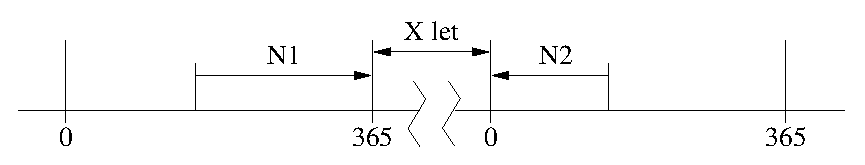
\includegraphics[scale=0.8]{img/datum1.eps}
  \caption{Řešení s~postupným výpočtem počtu dní mezi zadanými daty. N1
  reprezentuje počet dní od prvního zadaného data do konce roku, N2 je počet
  dní od začátku roku do druhého zadaného data a X je počet celých let mezi
  zadanými daty.}
  \label{fig:datum1}
\end{figure}

Obrázek \ref{fig:datum1} demonstruje první možnost výpočtu rozdílu dat. Nejprve
vypočteme počet dní od menšího data do konce roku, potom počet dní od začátku
druhého roku do druhého zadaného data. Poté zjistíme, kolik let leží mezi
zadanými daty a přepočítáme je na počet dnů. Součet těchto tří údajů dá
požadovaný rozdíl. 

\begin{figure}
  \centering
  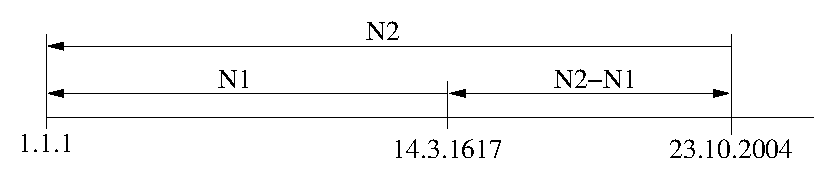
\includegraphics[scale=1]{img/datum2.eps}
  \caption{Řešení s~výpočtem dní od počátku letopočtu.}
  \label{fig:datum2}
\end{figure}

Druhou možností (obrázek \ref{fig:datum2}) je vypočítat u~každého data počet
dnů od počátku letopočtu do tohoto data a tyto dva údaje odečíst.

Při bližším prozkoumání obou možností se ukázalo, že první varianta není pro
výpočet rozdílu příliš vhodná, protože vyžaduje ošetření příliš mnoha
výjimečných stavů. Tímto výjimeč\-ným stavem je například situace, kdy obě data
leží ve stejném roce. Dalším zdrojem výjimečných stavů jsou přestupné dny
v~roce, které se mohou vyskytnout uvnitř nebo vně počítaných intervalů, což
vyžaduje ošetření hned čtyř možností. Druhá varianta výpočtu je mnohem
výhodnější i s~ohledem na započítávání přestupných let, protože obě data lze
před vlastním odečtením zpracovat naprosto stejným způsobem\footnote{Výpočet
počtu dnů od začátku letopočtu bude stejný pro obě data, nezávisle na tom,
které je starší.}, což vede na jediný podprogram. Z~těchto důvodů jsem
implementoval tuto druhou variantu.

%%%%%%%%%%%%%%%%%%%%%%%%%%%%%%%%%%%%%%%%%%%%%%%%%%%%%%%%%%%%%%%%%%%%%%%%%%%%%%
\section{Návrh řešení problému} \label{navrh}
%%%%%%%%%%%%%%%%%%%%%%%%%%%%%%%%%%%%%%%%%%%%%%%%%%%%%%%%%%%%%%%%%%%%%%%%%%%%%%

Po analýze problému s~počátkem letopočtu a počátkem gregoriánského kalendáře
jsem se rozhodl pro akceptování všech dat od počátku letopočtu (tedy od 1.1.1),
jako by se i~na ně tento kalendář vztahoval. Výpočet zahrnující i~počátek
gregoriánského kalendáře by totiž vyžadoval zadání údaje o~zeměpisné poloze
místa, pro které se tento výpočet provádí.

%=============================================================================
\subsection{Volba rozsahu}\label{rozsah}

Předpokládám, že datový typ \texttt{int} má na dnešních počítačích alespoň 32
bitů. Pokud by bylo potřeba aplikaci přenést na platformu s~menší délkou slova,
bude potřeba zvolit větší datové typy nebo zmenšit rozsah akceptovatelných dat.
Maximální hodnota typu \texttt{int} bez znaménka je 4294967296. Když tuto
hodnotu vydělíme délkou astronomického roku, vyjde maximální počet let
zobrazitelných pomocí počtu dnů 11759231. Nakonec jsem vybral hodnotu
maximálního akceptovatelného roku 11000000, protože je pro uživatele dobře
zapamatovatelná a obsahuje i dostatečnou rezervu hodnot proti případnému
přetečení.

%=============================================================================
\subsection{Výpočet rozdílu}

Princip zvoleného řešení je na obrázku \ref{fig:datum2}. V~tomto obrázku ovšem
není vyřešen problém se zahrnutím přechodných let. Zvolil jsem takové řešení,
že se nejprve počítá počet dnů od počátku letopočtu do zadaného data, přičemž
se neberou přestupné roky v~úvahu.  K~tomuto údaji se přičte počet přestupných
let mezi počátkem letopočtu a zadaným datem. Výsledkem je počet dnů od počátku
letopočtu včetně přestupných let. Před vlastním výpočtem rozdílu je potřeba
správně přehodit hodnoty, aby výsledek nevyšel záporně, protože výpočet probíhá
v~bezznaménkových číslech.

\paragraph*{Poznámka:} Protože jde o~počítání rozdílu dat, počítá se počet dnů
od počátku fiktivního roku nula. Výpočet se tím zjednoduší, protože není
potřeba neustále odečítat 365 dní.

\subsection{Výpočet přechodných let} Pro navržený algoritmus je potřeba vzorec
pro výpočet počtu přechodných let od počátku letopočtu. V~tomto vzorci se
uplatní všechna tři pravidla pro detekci přestupných let. Pro výpočet počtu dní
od roku 0 do konce zadaného roku jsem navrhnul tento vzorec:
\begin{equation}\label{eq:dni} dni = 365 * rok + \frac{rok}{4} -
\frac{rok}{100} + \frac{rok}{400} \end{equation}

Podmínku pro detekci, zda je rok přestupný, lze vytvořit pomocí operace modulo
(\%): 
\begin{equation}\label{eq:prestupny}
prestupny = (rok \% 4 == 0) \&\& ((rok \% 100 != 0) || (rok \% 400 == 0))
\end{equation}

%=============================================================================
\subsection{Analýza vstupních dat}

V~zadání je přesně specifikován formát vstupních dat včetně oddělovačů mezi
jednotlivými složkami jednotlivých dat.  V~jazyce C lze tento typ formátovaných
dat analyzovat pomocí funkce \texttt{scanf}, takže je zbytečné vymýšlet
speciální algoritmus. Po zavolání funkce \texttt{scanf} je potřeba detekovat
případné chyby rozsahu (např. datum menší než 1.1.1) a detekovat nesmyslné
datumy (např. 29.2.2003, 32.18.2000, atd.)

%=============================================================================
\subsection{Specifikace testů} \label{testy}

Z~návrhu řešení vyplývá několik rizikových oblastí, které je potřeba otestovat
-- chybný rozsah vstupních hodnot, chybně zadané datum (neodpovídá předepsané
syntaxi), nesmyslné datum a~chyby při výpočtu (hlavně s~přestupnými roky).

\paragraph{Test 1:} Chybná syntaxe $\longrightarrow$ Detekce chyby.
\begin{verbatim}
01.01.2000+02.01.2000
01,01,2000-02,01,2000
02 . 01 . 2000 - 1 . 1 . 2000
aleluja
\end{verbatim} 

\paragraph{Test 2:} Nesmyslná data $\longrightarrow$ Detekce chyby.
\begin{verbatim}
29.02.2001-29.2.2000
01.15.2001-31.4.2000
\end{verbatim} 

\paragraph{Test 3:} Data mimo povolený rozsah hodnot $\longrightarrow$ Detekce
chyby.
\begin{verbatim}
1.15.2001-15.2.0
1.1.1-31.12.110000001
\end{verbatim} 

\paragraph{Test 4:} Správnost výpočtu $\longrightarrow$ Předpokládaná správná
hodnota.

\vspace{1em}\begin{tabular}{ll} % ll = 2 sloupce zarovnane: left,left
vstup & očekávaný výstup \\
\hline
\verb|02.01.2000-1.1.2000| & 1 \\
\verb|1.1.2000-01.01.2000| & 0 \\
\verb|28.02.2000-28.2.2001| & 366 \\
\verb|29.2.2000-28.02.2001| & 365 \\
\verb|29.02.2000-1.03.2001| & 366 \\
\verb|1.03.2000-28.02.2001| & 364 \\
\verb|01.03.2001-29.02.2000| & 366 \\
\verb|31.12.11000000-15.10.1582| & 4017089764 \\
\verb|31.12.11000000-1.1.1| & 4017667499 \\
\verb|17.00004.1978-7.3.24063| & 8066340 \\
\end{tabular}


%%%%%%%%%%%%%%%%%%%%%%%%%%%%%%%%%%%%%%%%%%%%%%%%%%%%%%%%%%%%%%%%%%%%%%%%%%%%%%
\section{Popis řešení} \label{reseni}
%%%%%%%%%%%%%%%%%%%%%%%%%%%%%%%%%%%%%%%%%%%%%%%%%%%%%%%%%%%%%%%%%%%%%%%%%%%%%%

Při implementaci jsem vycházel ze závěrů popsaných v předchozích kapitolách.
Vlastní výpočet rozdílu dvou dat je implementován podle vzorců \ref{eq:dni} a
\ref{eq:prestupny}.

%=============================================================================
\subsection{Ovládání programu}

Program funguje jako konzolová aplikace, má tedy pouze textové ovládání. Při
spouštění program reaguje na jediný parametr \texttt{-h}. Pokud je s~tímto
parametrem zavolán, neprovádí žádný výpočet, ale vypíše obrazovku s~nápovědou.

Po spuštění program očekává na standardním vstupu řádek s~údaji v~zadaném
formátu. Pokud tam tento řetězec nenalezne, nebo pokud není dodržen vstupní
formát, vypíše chybové hlášení. To se vypíše i~v~případě, že zadaná data sice
syntakticky odpovídají požadavkům, ale představují neexistující datum. V
případě korektního vstupu se vypíše výsledný počet dnů na jediný řádek.

Výhodou takto strohého ovládání je, že program může být použit ve skriptech
(dávkových souborech) a~jím produkovaný výsledek může být použit jiným
programem pro další výpočet.

%=============================================================================
\subsection{Volba datových typů}

Pro uložení hodnot výsledku jsem zvolil datový typ \texttt{unsigned int} (viz
\ref{rozsah}). Pro uložení jednotlivých dat slouží struktura \texttt{TDate},
která obsahuje tři položky typu \texttt{unsigned int} pro den, měsíc a rok.
Datum je ve své podstatě heterogenní útvar, takže by nebylo vhodné ukládat jej
například do pole. Struktura navíc poskytuje prostor pro případné budoucí
rozšíření například o~časový údaj.

%=============================================================================
\subsection{Vlastní implementace}

Parametry příkazové řádky zpracovává funkce \texttt{doParams}, která je
spouštěna jako první ve funkci \texttt{main}. Poté se ze standardního vstupu
přečte textový řetězec se zadanými daty a předá se funkci \texttt{readDates}.
Ta pomocí volání \texttt{scanf} analyzuje vstupní řetězec a~detekuje v~něm
případné chyby. V~případě, že je vstup v~pořádku, naplní dvě struktury
\texttt{TDate}, které vrátí pomocí parametrů předávaných odkazem. Pro
otestování správnosti zadaných dat se volá funkce \texttt{isDateOk}, která
vrací logickou hodnotu.

Pro vlastní výpočet rozdílu slouží funkce \texttt{getDiff}, která dvakrát
zavolá funkci \texttt{getDays} a provede odečtení. Funkce \texttt{getDays}
pomocí funkcí \texttt{getDaysToYear}, \texttt{isLeapYear} vypočte podle výše
popisovaného vzorce počet dní od roku nula. Pro výpočet počtu dní od počátku
roku do zadaného data slouží tabulka (pole) \texttt{daysToMonth}, která
obsahuje dvanáct hodnot, jež představují počet dní od začátku roku do začátků
všech dvanácti měsíců.

%%%%%%%%%%%%%%%%%%%%%%%%%%%%%%%%%%%%%%%%%%%%%%%%%%%%%%%%%%%%%%%%%%%%%%%%%%%%%%
\section{Závěr} \label{zaver}
%%%%%%%%%%%%%%%%%%%%%%%%%%%%%%%%%%%%%%%%%%%%%%%%%%%%%%%%%%%%%%%%%%%%%%%%%%%%%%

Program počítá s~daty od začátku letopočtu podle gregoriánského kalendáře.
Kvůli výše zmíně\-ným problémům identifikací jeho počátečního data, nebylo do
řešení zahrnuto omezení na data mladší než rok 1582 (1583, 1700, ...) --
ostatně zadání nic takového nepožaduje. Tyto problémy by mohly být řešeny
v~dalších verzích programu jako volitelná rozšíření. Pravděpodobně by bylo
nutné pomocí parametru zadat místo, pro které se výpočet uskuteční. I tak by to
ale mělo smysl pouze pro oblasti, kde gregoriánský kalendář nahradil kalendář
juliánský. V jiných oblastech se používaly, či používají kalendáře, v nichž
implementovaný formát zápisu data nemá smysl.

Program byl úspěšně otestován v~prostředí operačních systémů Gnu/Linux a
MS~Windows se všemi navrženými testovacími hodnotami.  Program přesně dodržuje
požadavky kladené na formát vstupních a výstupních dat, takže může být
bezproblémově používán spolu s~dalšími programy ve skriptech nebo jiných
programech.

Navržené řešení je přenositelné na všechny platformy, pro které
platí \texttt{sizeof(int)} $\geq 4$. Pro přenos na platformu s~menší velikostí
datového typu \texttt{int} by bylo nutné buďto zmenšit rozsah akceptovatelných
dat nebo upravit datové typy, které se používají při výpočtu.

%%%%%%%%%%%%%%%%%%%%%%%%%%%%%%%%%%%%%%%%%%%%%%%%%%%%%%%%%%%%%%%%%%%%%%%%%%%%%%
% seznam citované literatury: každá položka je definována příkazem
% \bibitem{xyz}, kde xyz je identifikátor citace (v textu použij: \cite{xyz})
\begin{thebibliography}{1}

% jedna citace:
\bibitem{kalendar}
BLACKBURN, B.~J.; HOLFORD-STREVENS, L.: \emph{The Oxford Companion to the
  Year}. Oxford: Oxford University Press, 1999, ISBN 0-19-214231-3.


\end{thebibliography}
%%%%%%%%%%%%%%%%%%%%%%%%%%%%%%%%%%%%%%%%%%%%%%%%%%%%%%%%%%%%%%%%%%%%%%%%%%%%%%
% přílohy
\appendix

\section{Metriky kódu} \label{metriky}
\paragraph{Počet souborů:} 1 soubor
\paragraph{Počet řádků zdrojového textu:} 238 řádků
\paragraph{Velikost statických dat:} 3328B
\paragraph{Velikost spustitelného souboru:} 9434B (systém Linux, 32 bitová
architektura, při překla\-du bez ladicích informací)


\end{document}
